\chapter{Zaimplementowane elementy maszyny wirtualnej}
\label{cha:maszyna}

W rozdziale wymieniono elementy maszyny wirtualnej Erlanga rozważanej w pracy z uwzględnieniem 
opisu sposobu działania poszczególnych elementów, ich roli w maszynie wirtualnej, a także porównania
funkcjonalności do maszyny wirtualnej BEAM.

%---------------------------------------------------------------------------
\section{Moduł ładujący kod (\emph{loader})}
\label{sec:maszynaLoader}

%---------------------------------------------------------------------------
\section{Typy danych}
\label{sec:maszynaTypy}

%---------------------------------------------------------------------------
\section{Tablice}
\label{sec:maszynaTablice}

Biorąc pod uwagę modułowy charakter aplikacji napisanych w języku Erlang, maszyna wirtualna musi posiadać pewien mechanizm pozwalający na utrzymywanie globalnego stanu systemu w zależności od aktualnie załadowanych modułów.

Strukturą danych przeznaczoną do tego celu jest tablica z haszowaniem wspomagana przez tablicę indeksów. Połączenie tych dwóch struktur umożliwia wstawienie nowego elementu oraz sprawdzenie jego indeksu w czasie stałym (konieczne jest wyliczenie skrótu). W takim samym czasie (nie jest do tego jednak konieczne wyliczanie skrótu) możliwe jest znalezienie obiektu znając jego indeks. Co więcej, w reprezentacji kodu maszynowego posługiwanie się indeksami obiektów trywializuje ich porównywanie czy pobieranie ich wartości w trakcie jego wykonywania.

Wybór takiej struktury danych ma więc charakter optymalizacyjny. W maszynie wirtualnej tablicowanymi obiektami są: \textbf{atomy} i \textbf{eksportowane funkcje}. Maszyna wirtualna BEAM dodatkowo tablicuje również \textbf{moduły}, gdzie przechowywane są informacje o wskaźnikach do początku kodu modułu w dwóch wersjach: nowej i starej, które mogą działać w maszynie wirtualnej niezależnie od siebie. Ponieważ jednak maszyna rozważana w pracy w obecnej fazie rozwoju nie zapewnia możliwości dynamicznego ładowania modułów, struktura ta nie jest konieczna.

Na rysunku \ref{fig:atomtable} przedstawiono sposób w jaki wewnątrz maszyny wirtualnej przechowywane są stablicowane dane.  Przykład ten dotyczy dwuelementowej tablicy atomów, które były do niej wstawiane w kolejności: \texttt{erlang}, \texttt{+}. Strzałki na diagramie reprezentują przechowywanie wskaźników na struktury atomów przez tablice: z haszowaniem i indeksów.

\begin{figure}[h]
\centerline{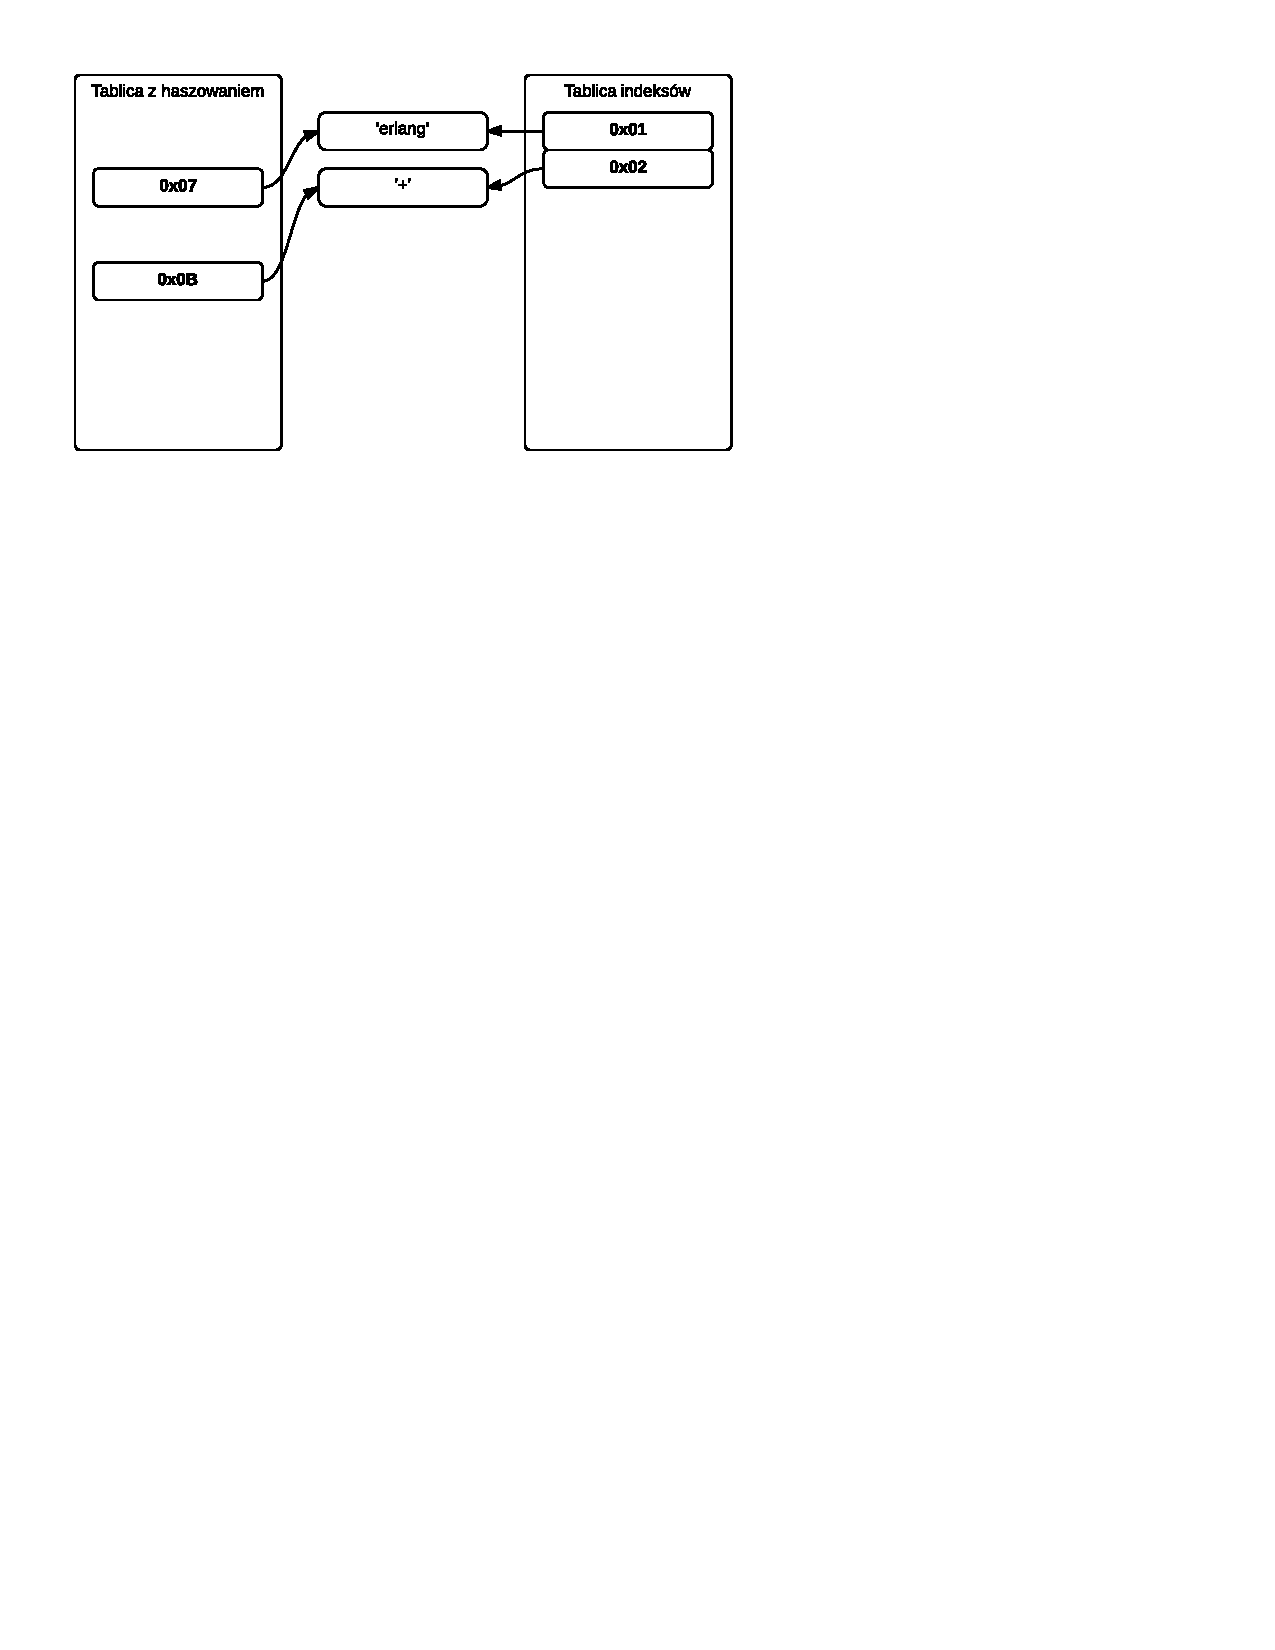
\includegraphics[scale=1, clip, trim=0 200mm 90mm 0]{atom_table}}
\caption{Przykład przechowywania danych stablicowanych danych wewnątrz maszyny wirtualnej.}
\label{fig:atomtable}
\end{figure}

W maszynie BEAM, w przypadku uruchomionych dużych systemów, powyższe struktury danych mogą zawierać bardzo dużą liczbę elementów, nawet rzędu kilkudziesięciu tysięcy. Zupełnie inaczej sytuacja wygląda w niniejszej maszynie wirtualnej ze względu na jej przeznaczenie - systemy wbudowane oraz restrykcyjne limity dostępnej pamięci RAM. Rozmiary tablic nie powinny zatem przekraczać liczby elementów wyrażonej w setkach atomów czy funkcji eksportowanych. Niemniej jednak, ze względu na możliwość uruchomienia systemu FreeRTOS na mikrokontrolerach o różnych parametrach, pozostawiono możliwość zdefiniowania maksymalnej liczby elementów, jakie mogą zostać wstawione do tablic. Zaimplementowano również mechanizmy automatycznego rozszerzania tablic wraz ze wzrostem liczby elementów, w celu optymalizacji pamięci zajmowanej przez tablice.

Ważną cechą charakterystyczną tablic w maszynie wirtualnej jest również fakt, że raz wstawionego do nich obiektu nie można z niej usunąć. W kontekście maszyny wirtualnej rozważanej w pracy ta cecha nie ma większego znaczenia, gdyż obecnie nie umożliwia ona dynamicznego ładowania modułów po jej uruchomieniu. Jednak w przypadku maszyny BEAM nie należy zapominać o tej cesze np. w sytuacji, gdy program dynamicznie generuje atomy. Tablica atomów w BEAM może przechowywać aż 1048576 atomów, należy jednak mieć na uwadze to, że próba dodania atomu do pełnej już tablicy zakończy się zakończeniem procesu maszyny wirtualnej.

%---------------------------------------------------------------------------
\subsection{Tablica atomów}
\label{sub:maszynaTablicaAtomow}

Funkcja skrótu dla atomów (ich reprezentacji w postaci napisu) używana w maszynie wirtualnej to \emph{hashpjw} \cite{Aho1986}. Jest to funkcja o bardzo dobrym rozkładzie wartości skrótu dla napisów, jednak wartość zwracana przez oryginalną funkcję jest 32-bitowa.

W celu ograniczenia pamięci zajmowanej przez tablice w maszynie wirtualnej rozważanej w pracy, funkcja haszująca została zmodyfikowana tak, aby zwracała wynik 8-bitowy. Ze względu na duże różnice w rozmiarach tablic pomiędzy rozważaną maszyną a BEAM zmniejszenie długości skrótu zwracanego z funkcji haszującej nie będzie miało wpływu na liczbę kolizji w tablicy z haszowaniem. 

Źródłem atomów w tablicy są atomy zdefiniowane w samej maszynie wirtualnej oraz atomy pochodzące z ładowanych modułów. Atomy zdefiniowane ładowane są do tablicy w trakcie uruchamiania maszyny wirtualnej w określonej kolejności, co za tym idzie atomy te mają z góry ustalony i znany indeks, co jest wykorzystywane np. przy definicji funkcji wbudowanych w maszynę wirtualną (por. \ref{sec:maszynaBIF}). Z kolei indeksy atomów, które pochodzą z ładowanych modułów, a nie zostały wcześniej zdefiniowane, przydzielane są w kolejności ładowania modułów i występowania atomów w tablicach atomów modułów. Równość dwóch atomów oznacza zawsze równość ich indeksów w globalnej tablicy atomów i na odwrót, niezależnie od źródła ich pochodzenia ani momentu załadowania modułu do maszyny wirtualnej.

%---------------------------------------------------------------------------
\subsection{Tablica eksportowanych funkcji}
\label{sub:maszynaTablicaEksportow}

Funkcja skrótu dla eksportowanych funkcji ma wartość $M \cdot F+A$, gdzie $M$ to indeks w tablicy atomów dla nazwy modułu z którego eksportowana jest funkcja, $F$ to indeks w tablicy atomów dla nazwy eksportowanej funkcji, a $A$ to arność tej funkcji.

Wpisy w tablicy eksportowanych funkcji pochodzą z modułów załadowanych do maszyny wirtualnej, dla funkcji które zostały zdefiniowane w lokalnej tablicy eksportów dla danego modułu. W takiej sytuacji w tablicy eksportów przechowywany jest wskaźnik na miejsce w pamięci, w którym znajduje się pierwsza instrukcja funkcji. Interpreter, wykonując kod używa indeksu do odczytania adresu tej instrukcji, a następnie wykonuje skok do tego miejsca pamięci i kontynuuje wykonywanie kodu, po uprzednim zapisaniu adresu powrotu.

Elementy tablicy mogą pochodzić również z wbudowanych funkcji (por. \ref{sec:maszynaBIF}). W tym przypadku, tablica eksportów zawiera wskaźnik do funkcji w języku C, zaimplementowanej jako część maszyny wirtualnej, która zostanie wykonana przez interpreter.

Ponieważ równość indeksów w tablicy eksportów jest równoważna z równością trójek $\lbrace\text{moduł},\text{funkcja},\text{arność}\rbrace$, w sytuacji dynamicznej podmiany kodu nie jest konieczna zmiana indeksu w załadowanym do pamięci kodzie maszynowym, a tylko odpowiednia zmiana struktury znajdującej się pod tym indeksem.

%---------------------------------------------------------------------------
\section{Interpreter kodu maszynowego}
\label{sec:maszynaInterpreter}

%---------------------------------------------------------------------------
\section{Procesy}
\label{sec:maszynaProcesy}

%---------------------------------------------------------------------------
\section{Planista (\emph{scheduler})}
\label{sec:maszynaScheduler}

%---------------------------------------------------------------------------
\section{Funkcje wbudowane (\emph{Built-In Functions})}
\label{sec:maszynaBIF}

%---------------------------------------------------------------------------
\section{\emph{Garbage collector}}
\label{sec:maszynaGC}

%---------------------------------------------------------------------------
\section{Mechanizmy zarządzania czasem}
\label{sec:maszynaTimer}